%!TEX root = Slides.tex
\section{Anwendungsf\"alle}

\begin{frame}[t]
\frametitle{\insertsection}
\structure{\textbf{Auftragsmanagement}}\\[4pt]
\structure{\textbf{Universit\"atsverwaltung}}\\[8pt]
\begin{itemize}
	\item Arbeit in kleinen Teams
	\item Erstellen von ER-Modellen und relationalen Modellen
	\item Implementierung in SQL
	\item Datengenerierung
	\item Abfragen in Datenbank
	\item Pr\"asentation der Ergebnisse durch die Teams
\end{itemize}
\end{frame}

\subsection*{Auftragsmanagement}

\begin{frame}[t]
\frametitle{\insertsection}
\framesubtitle{\insertsubsection}
\structure{In einem Unternehmen existieren \emph{Kunden} und \emph{Mitarbeiter}}
\begin{itemize}
\item Kunden und Mitarbeiter werden mit Vor- und Nachnamen erfasst 
\item Kunden und Mitarbeitern wird eine \textit{Adresse} zugeordnet
\begin{itemize}
	\item Eine Adresse besteht aus Stra\ss e, Postleitzahl und Ort
	\item Beschr\"ankung auf inl\"andische Adressen, die nach diesem Schema aufgebaut sind
\end{itemize}
\item Bei Kunden wird zus\"atzlich das Datum festgehalten, seitdem er Kunde ist 
\item Weiterhin wird beim Kunden hinterlegt, \textit{welcher Mitarbeiter den Kunden angelegt hat} 
\item Bei Mitarbeitern wird das Gehalt und das erste Anstellungsdatum hinterlegt. 
\end{itemize}
\end{frame}

\begin{frame}[t]
\frametitle{Anwendungsf\"alle}
\framesubtitle{\insertsubsection}
	\structure{Das Unternehmen verkauft \emph{Produkte}, die in \emph{Produktgruppen} unterteilt sind}
	\begin{itemize}
		\item Eine Produktgruppe kann mehrere Produkte beinhalten 
		\item Jedes Produkt wird genau einer Produktgruppe zugeordnet 
		\item Eine Produktgruppe besteht lediglich aus einer \textit{Bezeichnung} 
		\item Zu einem Produkt werden ebenfalls eine \textit{Bezeichnung} und ein \textit{Nettopreis} hinterlegt
	\end{itemize}
  \abs 
	\structure{Kunden können \emph{Auftr\"age} abgeben}
	\begin{itemize}
		\item Zu jedem Auftrag wird das \emph{Datum}, der zuständige Mitarbeiter und der betreffende Kunde hinterlegt 
		\item Jeder Auftrag umfasst \emph{Auftragspositionen}, das entsprechende Produkt sowie die beauftragte \emph{Menge} des Produktes
	\end{itemize}
\end{frame}
	
\begin{frame}[t]
\frametitle{Anwendungsf\"alle}
\framesubtitle{\insertsubsection}
		\begin{alertblock}{Aufgabenstellung}
			\begin{enumerate}
				\item Erstellen Sie ein ER-Modell für den Anwendungsfall
				\item Erstellen Sie aus dem ER-Modell das logische Datenmodell 
				\item Implementieren Sie das Datenmodell auf der PostgreSQL-Datenbank 
				\item Befüllen Sie die Datenbank mit ausreichend vielen Testdaten 
			\end{enumerate}
		\end{alertblock}
\end{frame}

\begin{frame}[t]
\frametitle{Anwendungsf\"alle}
\framesubtitle{\insertsubsection}
\begin{alertblock}{Aufgabenstellung (Fortsetzung)}
	\begin{enumerate}
		\setcounter{enumi}{4}
		\item\label{A1} Erstellen Sie eine Abfrage, welche alle Aufträge mit den zugehörigen Auftragspositionen, geordnet nach
		Auftragsnummer und Auftragspositionsnummer (in dieser Reihenfolge) ausgibt.
		\item\label{A2} Fragen Sie die nach Kunden gruppierte Anzahl aller Aufträge ab. Ausgegeben
		werden soll die Kundennummer, Vor- und Nachname sowie die Anzahl der abgegebenen Aufträge.
		\item\label{A3} Fragen Sie die Umsätze aller Aufträge nach Mitarbeitern gruppiert ab.
		\item\label{A4} Erstellen Sie eine Abfrage, welche die Personennummer, Vorname, Nachname und Umsatz derjenigen Mitarbeiter 
		mit Umsätzen von mehr als 5.000 Euro ausgibt.
		\item\label{A5} Fragen Sie die Anzahl aller Produkte innerhalb einer Produktgruppe ab.
	\end{enumerate}
\end{alertblock}
\end{frame}

\begin{frame}[t]
\frametitle{Anwendungsf\"alle}
\framesubtitle{\insertsubsection}
  \begin{alertblock}{Aufgabenstellung (Fortsetzung)}
		\begin{enumerate}
			\setcounter{enumi}{9}
			\item\label{A6} Erzeugen Sie eine Übersicht über alle Produktgruppen (PGID und Bezeichnung), in denen keine Produkte enthalten sind.					
			\item\label{A7} Erzeugen Sie eine Übersicht mit Personennummer, Vorname und Nachname von allen Personen, deren letzter Auftrag länger als 720 Tage zurückliegt.
			\item\label{A8} Ausgabe aller Kunden, die einen Bestellabstand zwischen zwei Bestellungen von mehr als 60 Tagen aufweisen. Ausgegeben werden soll
			 die Kundennummer, Vorname, Nachname, die beiden Datumsangaben derjenigen Bestellungen, die mehr als 60 Tage auseinander liegen sowie
			 die Differenz in Tagen.
		\end{enumerate}
	\end{alertblock}
\end{frame}

\subsection*{Universit\"atsverwaltung}

\begin{frame}[t]
\frametitle{Anwendungsf\"alle}
\framesubtitle{\insertsubsection}
\begin{figure}
	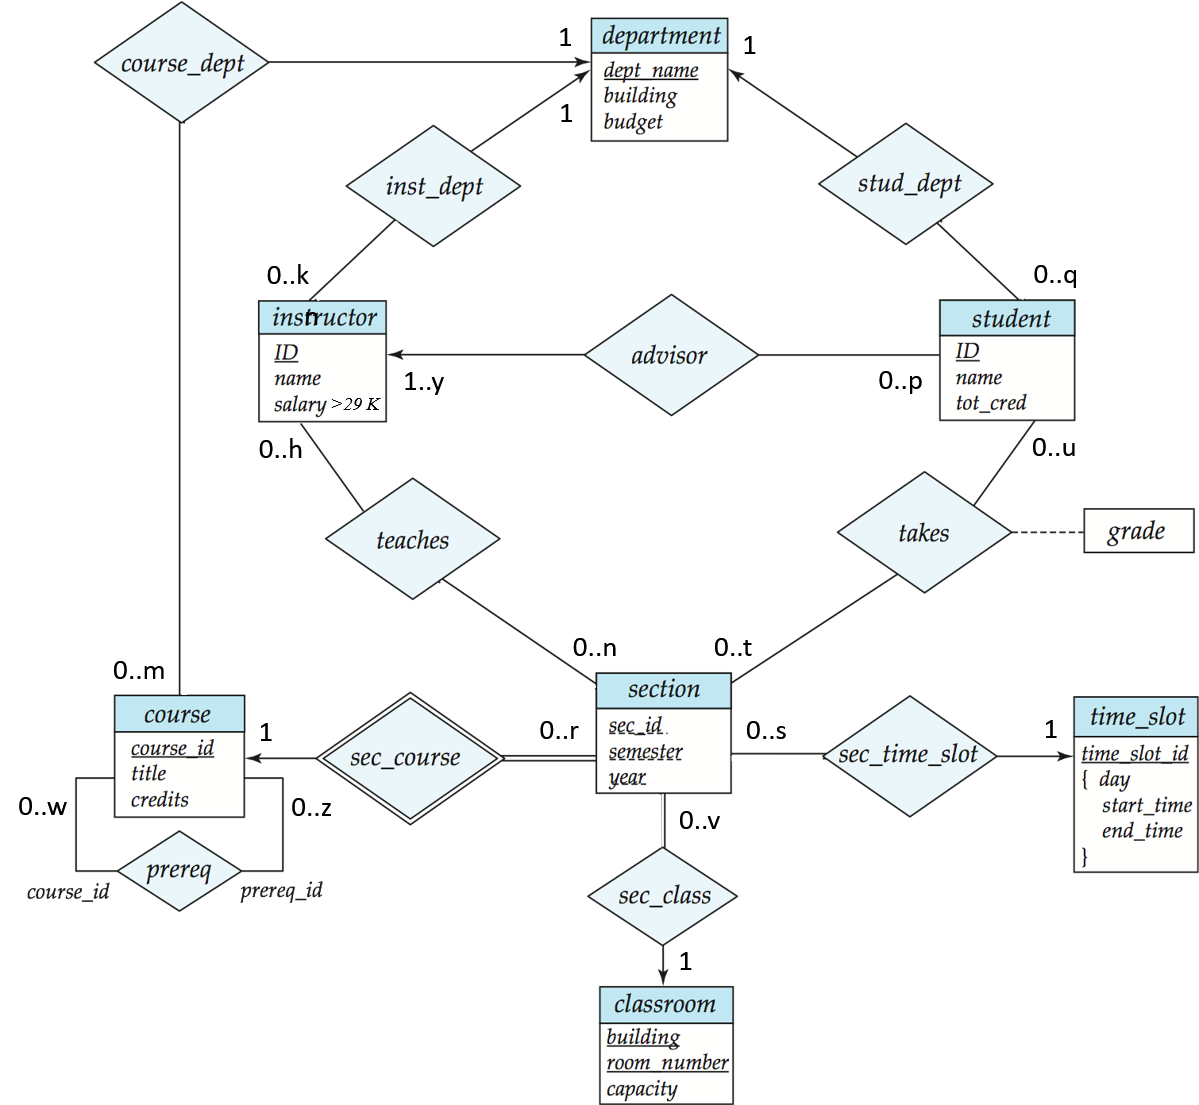
\includegraphics[scale=0.35]{img/ERM-UniversityUseCase.png}
\end{figure}
\end{frame}

\begin{frame}[t]
\frametitle{Anwendungsf\"alle}
\framesubtitle{\insertsubsection}
\begin{alertblock}{Aufgabenstellung}
\begin{enumerate}
	\item Erstellen Sie aus dem ER-Modell das logische Datenmodell 
	\item Implementieren Sie das logische Datenmodell auf der PostgreSQL-Datenbank 
	\item Befüllen Sie die Datenbank mit ausreichend vielen Testdaten aus dem Datenpool der Vorlesung
\end{enumerate}
\end{alertblock}
\abs
\abs
\textbf{Beachten Sie:} Das ER-Modell soll in seiner \"au\ss eren Struktur -- Entit\"aten, Beziehungen, Kardinalit\"aten -- realisiert 
werden. Die innere Struktur wie beispielsweise Anzahl, Art und Datentypen der Attribute k\"onnen Sie nach Ihren eigenen Ideen und
Vorstellungen entwerfen.
\end{frame}

\begin{frame}[t]
\frametitle{Anwendungsf\"alle}
\framesubtitle{\insertsubsection}
\begin{alertblock}{Aufgabenstellung (Fortsetzung)}
\begin{enumerate}
 \setcounter{enumi}{3}	
 % 2.2
 \item Betrachten Sie die Fremdschl\"usselbeziehung vom \texttt{dept\_name}-Attribute von der Relation der Dozenten 
  (\texttt{instructor}) auf die Fakult\"aten-Relation (\texttt{department}). Geben Sie Beispiele von Eingabe- 
  und L\"oschoperationen auf diesen Tabellen an, die eine Verletzung der Fremdschl\"usselbeziehung zur Folge haben.
 % 2.5
 \item\label{first} Was ist das Ergebnis der Hintereinanderausf\"uhrung folgender Operationen: 
  \begin{itemize} 
	 \item Kartesisches Produkt der Relationen \texttt{student} und \texttt{advisor} (und ggf.~\texttt{instructor}).
	 \item Selektion auf diesem Produkt mit der Bedingung \texttt{s\_id}$=$\texttt{i\_ID}? 
  \end{itemize}
  F\"uhren Sie die entsprechende SQL-Anweisung auf der Datenbank durch.
\end{enumerate}
\end{alertblock}
\end{frame}

\begin{frame}[t]
\frametitle{Anwendungsf\"alle}
\framesubtitle{\insertsubsection}
\begin{alertblock}{Aufgabenstellung (Fortsetzung)}
\begin{enumerate}
 \setcounter{enumi}{5}	
 % 2.6
 \item\label{U1} F\"uhren Sie folgende Operationen der relationalen Algebra in SQL auf der Datenbank aus.
  \"Uberlegen Sie sich vorab, welches Ergebnis die jeweilige Operation liefert.
  \begin{itemize}
   \item $\sigma_{year= 2009}(\texttt{section}\bowtie\texttt{takes})\bowtie\texttt{student}$
   \item $\sigma_{year= 2009}(\texttt{section}\bowtie\texttt{takes}\bowtie\texttt{student})$
   \item $\Pi_{ID,name,course\_id}(\texttt{section}\bowtie\texttt{takes}\bowtie\texttt{student})$
  \end{itemize}
 % 3.4
 \item\label{U2} F\"uhren Sie die folgenden Inserts, Updates, Deletes auf der Datenbank durch:
  \begin{itemize}
   \item Erh\"ohe das Gehalt jedes Dozenten in der Fakult\"at Informatik (\texttt{Comp. Sci.}) um 10\%.
   \item L\"osche alle Kurse, die nie angeboten wurden, d.~h., die nicht in der \texttt{section}-Tabelle vorkommen.
   \item F\"uge jede(n) Studierende(n) mit mehr als 100 Gesamt-Credit-Points (\texttt{tot\_cred}) in die 
    \texttt{instructor}-Tabelle mit einem Gehalt von 10.000 \$ ein. Vorsicht!
  \end{itemize}
\end{enumerate}
\end{alertblock}
\end{frame}

\begin{frame}[t]
\frametitle{Anwendungsf\"alle}
\framesubtitle{\insertsubsection}
\begin{alertblock}{Aufgabenstellung (Fortsetzung)}
\begin{enumerate}
 \setcounter{enumi}{7}	
 % 3.1 
 \item\label{U3} Dr\"ucken Sie die folgenden Anfragen in SQL aus und f\"uhren Sie die entsprechende Abfrage auf der 
  Datenbank durch:
  \begin{itemize}
   \item Finde die Kurse in der Fakult\"at Informatik (\texttt{Comp.~Sci.}) mit drei credit points.
   \item Finde die \texttt{ID}s aller Studenten, die Dozent (\texttt{instructor}) 
    \texttt{Bondi} unterrichtet. 
   \item Finde das h\"ochste Gehalt eines Dozenten. Finde alle Dozenten mit h\"ochstem Gehalt.
   \item Finde die Anzahl Einschreibungen in jeder Sektion (Tabelle \texttt{section}) eines Kurses im Wintersemester 
    (\texttt{Fall}) 2009.
   \item Finde die maximale Einschreibungszahl im Wintersemester (\texttt{Fall}) 2009.
   \item Finde die Sektionen mit maximaler Einschreibungszahl im Wintersemester (\texttt{Fall}) 2009.
  \end{itemize}
\end{enumerate}
\end{alertblock}
\end{frame}

\begin{frame}[t]
\frametitle{Anwendungsf\"alle}
\framesubtitle{\insertsubsection}
\begin{alertblock}{Aufgabenstellung (Fortsetzung)}
\begin{enumerate}
 \setcounter{enumi}{8}	
 % 4.1
 \item\label{U4} F\"uhren Sie folgende Anfragen auf der Datenbank aus: 
  \begin{itemize}
   \item Anzeige aller Dozenten mit ihren IDs, Namen und die Anzahl von Sektionen, die sie lehrten (Anzeige "0", falls 
    keine Sektion gelehrt wurde). 
   \item Anzeige aller Kombinationen von Sektionen, die im Sommersemester (\texttt{Spring}) 2010 angeboten wurden, 
    und den Namen der zugeh\"origen Dozenten. Wenn eine Sektion nicht gelehrt wurde, soll sie mit Dozentennamen 
    '\texttt{-}' ausgegeben werden.
   \item Anzeige aller Fakult\"aten (\texttt{department}) und der Gesamtzahl der zu der jeweiligen Fakult\"at
    geh\"orenden Dozenten. Auch Fakult\"aten ohne Dozenten sollen korrekt angezeigt werden.    	
  \end{itemize}
 % 4.2 
 \item\label{U5} Outer Joins k\"onnen in SQL ohne die explizite Verwendung der '\texttt{OUTER JOIN}'-Operation ausgef\"uhrt werden.
  Zeigen Sie das anhand der folgenden SQL-Anfragen:
  \begin{itemize}
   \item \texttt{SELECT * FROM student NATURAL LEFT OUTER JOIN takes}
   \item \texttt{SELECT * FROM student NATURAL FULL OUTER JOIN takes}
  \end{itemize}
\end{enumerate}
\end{alertblock}
\end{frame}

\begin{frame}[t]
\frametitle{Anwendungsf\"alle}
\framesubtitle{\insertsubsection}
\begin{alertblock}{Aufgabenstellung (Fortsetzung)}
\begin{enumerate}
 \setcounter{enumi}{10}	
 % 4.8
 \item\label{U6} Ein Dozent kann nicht zwei oder mehr Sektionen im gleichen time slot im Semester und Jahr unterrichten. 
  \begin{itemize}
   \item Schreiben Sie eine SQL-Abfrage, mit der alle (Dozent,Sektion)-Tupel bestimmt werden, die diese Bedingung verletzen
   \item \"Uberlegen Sie sich, wie diese Bedingung bereits in den Relationenschemata und den Integrit\"atsbedingungen
    festgelegt werden kann, um falsche Dateneingaben zu vermeiden.
  \end{itemize}
\end{enumerate}
\end{alertblock}
\end{frame}
